\chapter{Wiadukt WK2 w ciągu Pomorskiej Kolei Metropolitalnej}

\section{Charakterystyka obiektu}
Obiekt badawczy stanowi kolejowy wiadukt łukowy w ciągu linii Pomorskiej Kolei Metropolitalnej w km 1+696,02. Przęsło wiaduktu stanowi stalowy ustój łukowy z jazdą dołem. Główne wymiary charakteryzujące konstrukcję to: 
\begin{itemize}
	\item rozpiętość teoretyczna: $L_t=70.00 \text{m}$, 
	\item długość całkowita:  $L_c=71,60 \text{m}$, 
	\item wysokość w kluczu:  $H=11.00 !!! \text{m}$,
	\item szerokość całkowita: $B_c=10.21 \text{m}$. 
\end{itemize}
 Przekrój poprzeczny dźwigarów łukowych zaprojektowano jako skrzynkowy. Pomost wykonano jako ortotropowy, z blachy wzmocnionej żebrami podłużnymi i poprzecznicami o przekroju teowym. Poprzecznice rozmieszczono w rozstawie 2.5 m. Ściąg łuku stanowią belki dwuteowe, po jednej dla każdego dźwigara łukowego. Przekrój ściągu zmienia się z dwuteowego na skrzynkowy w strefie podporowej. W zrealizowanym wariancie pomost został podwieszony do łuku za pomocą prętowych, prostych wieszaków o średnicy 100 mm. Po każdej ze stron zamontowano 12 wieszaków w rozstawie co 5 m. Wieszaki zostały połączone z dźwigarem i ściągiem sztywnym połączeniem spawanym. Przekrój poprzeczny konstrukcji przęseł pokazano na rysunku (!!!). Widok na zrealizowane przęsło pokazano na rysunku \ref{fig: wk2_foto_widok_front}, detale konstrukcyjne w obrębie strefy podporowej zaprezentowano na rysunku \ref{fig:  wk2_foto_wezglowie}, a połączenie wieszaka ze ściągiem na rysunku \ref{fig: wk2_foto_wieszak}.

\begin{figure}[h]
	\centering
	\subfloat{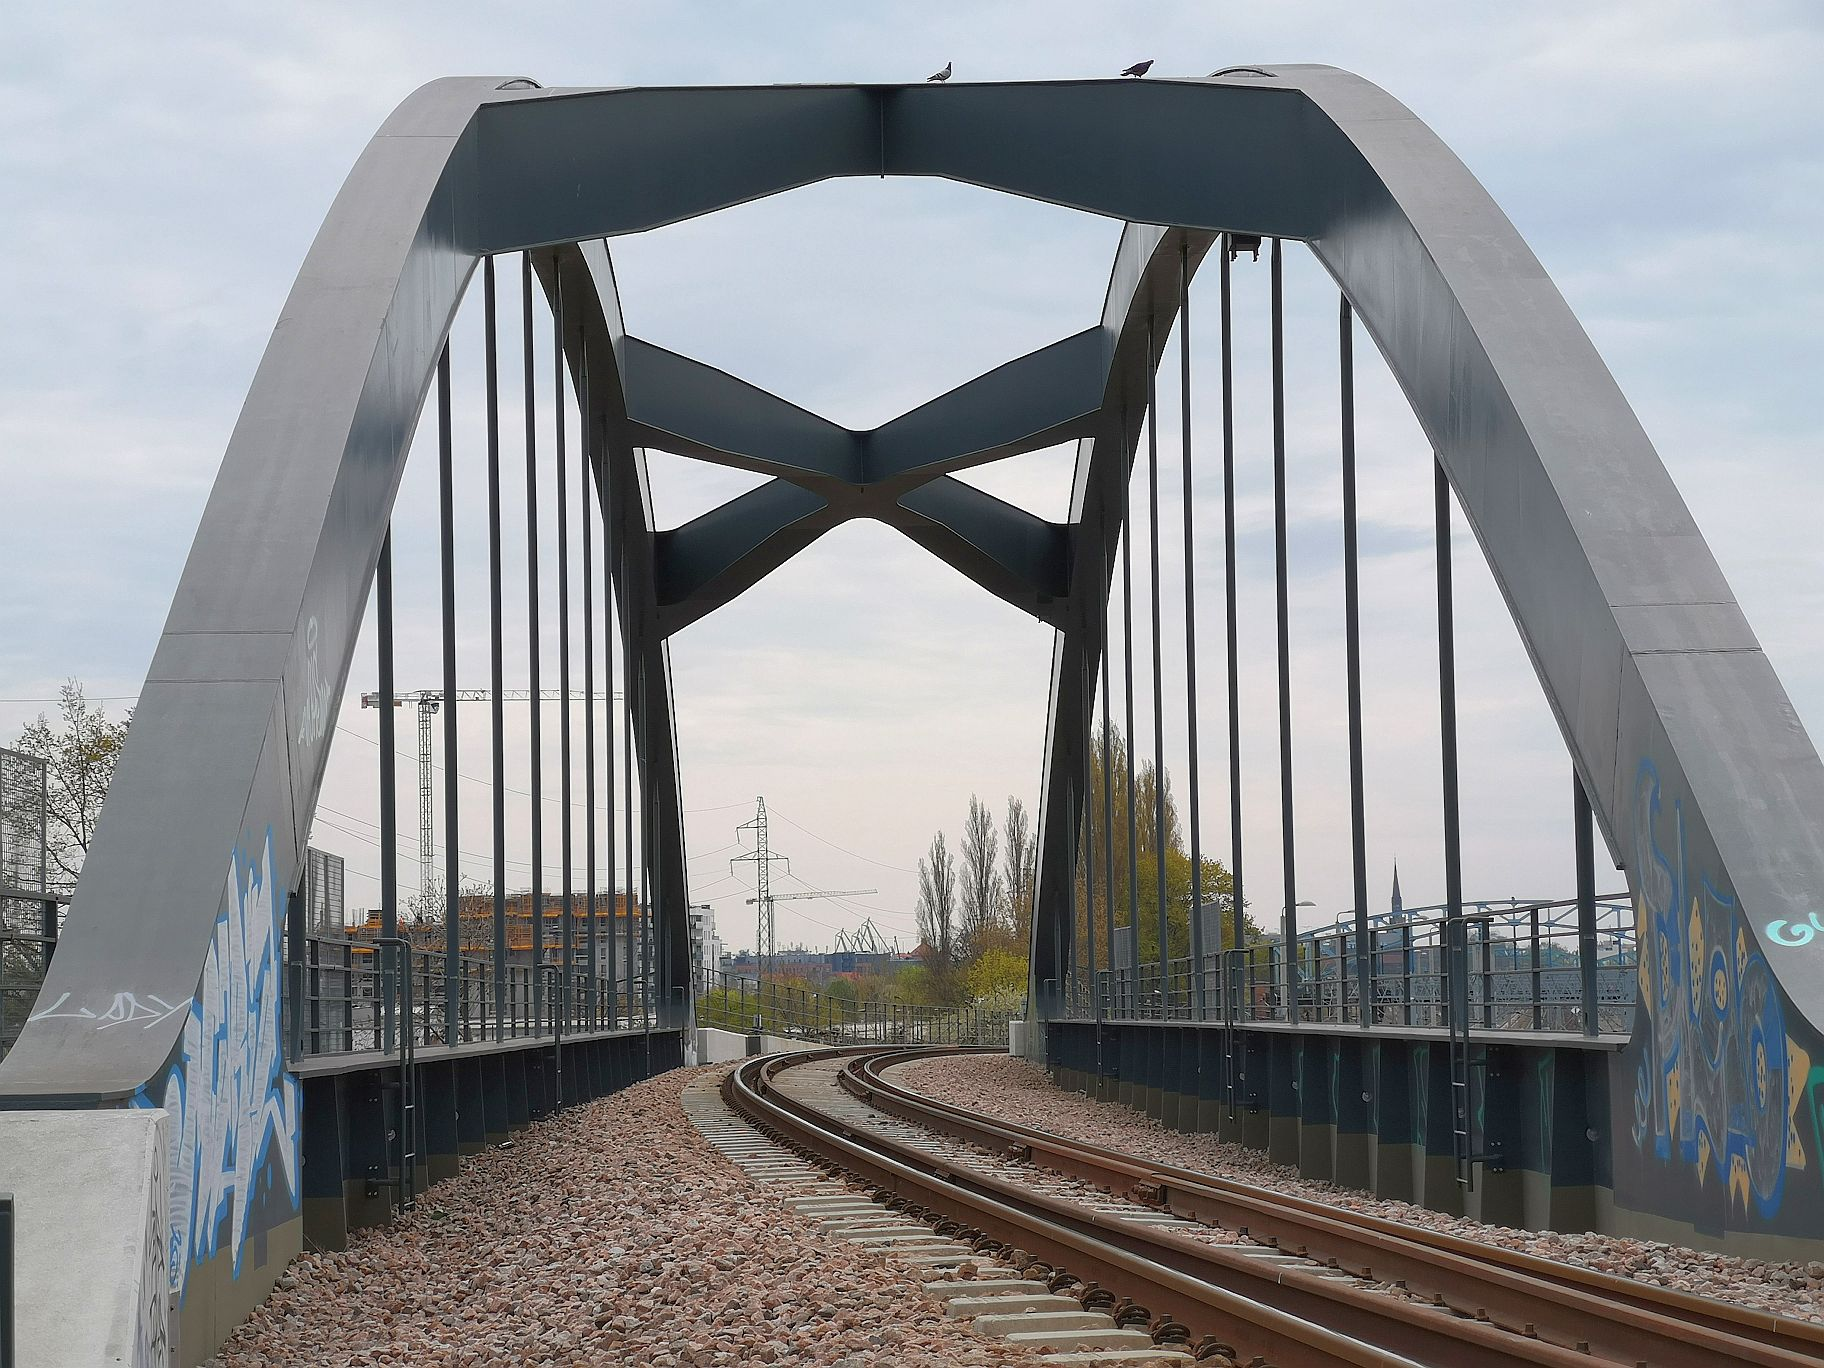
\includegraphics[height=0.35\textheight]{/WK2/zdjecia/widok_front2.jpg}} 
	\captionsetup{justification=centering}
	\caption{Widok od frontu na wiadukt WK2}
	\label{fig: wk2_foto_widok_front}
\end{figure}
\begin{figure}[h]
	\centering
	\subfloat[Widok z góry]{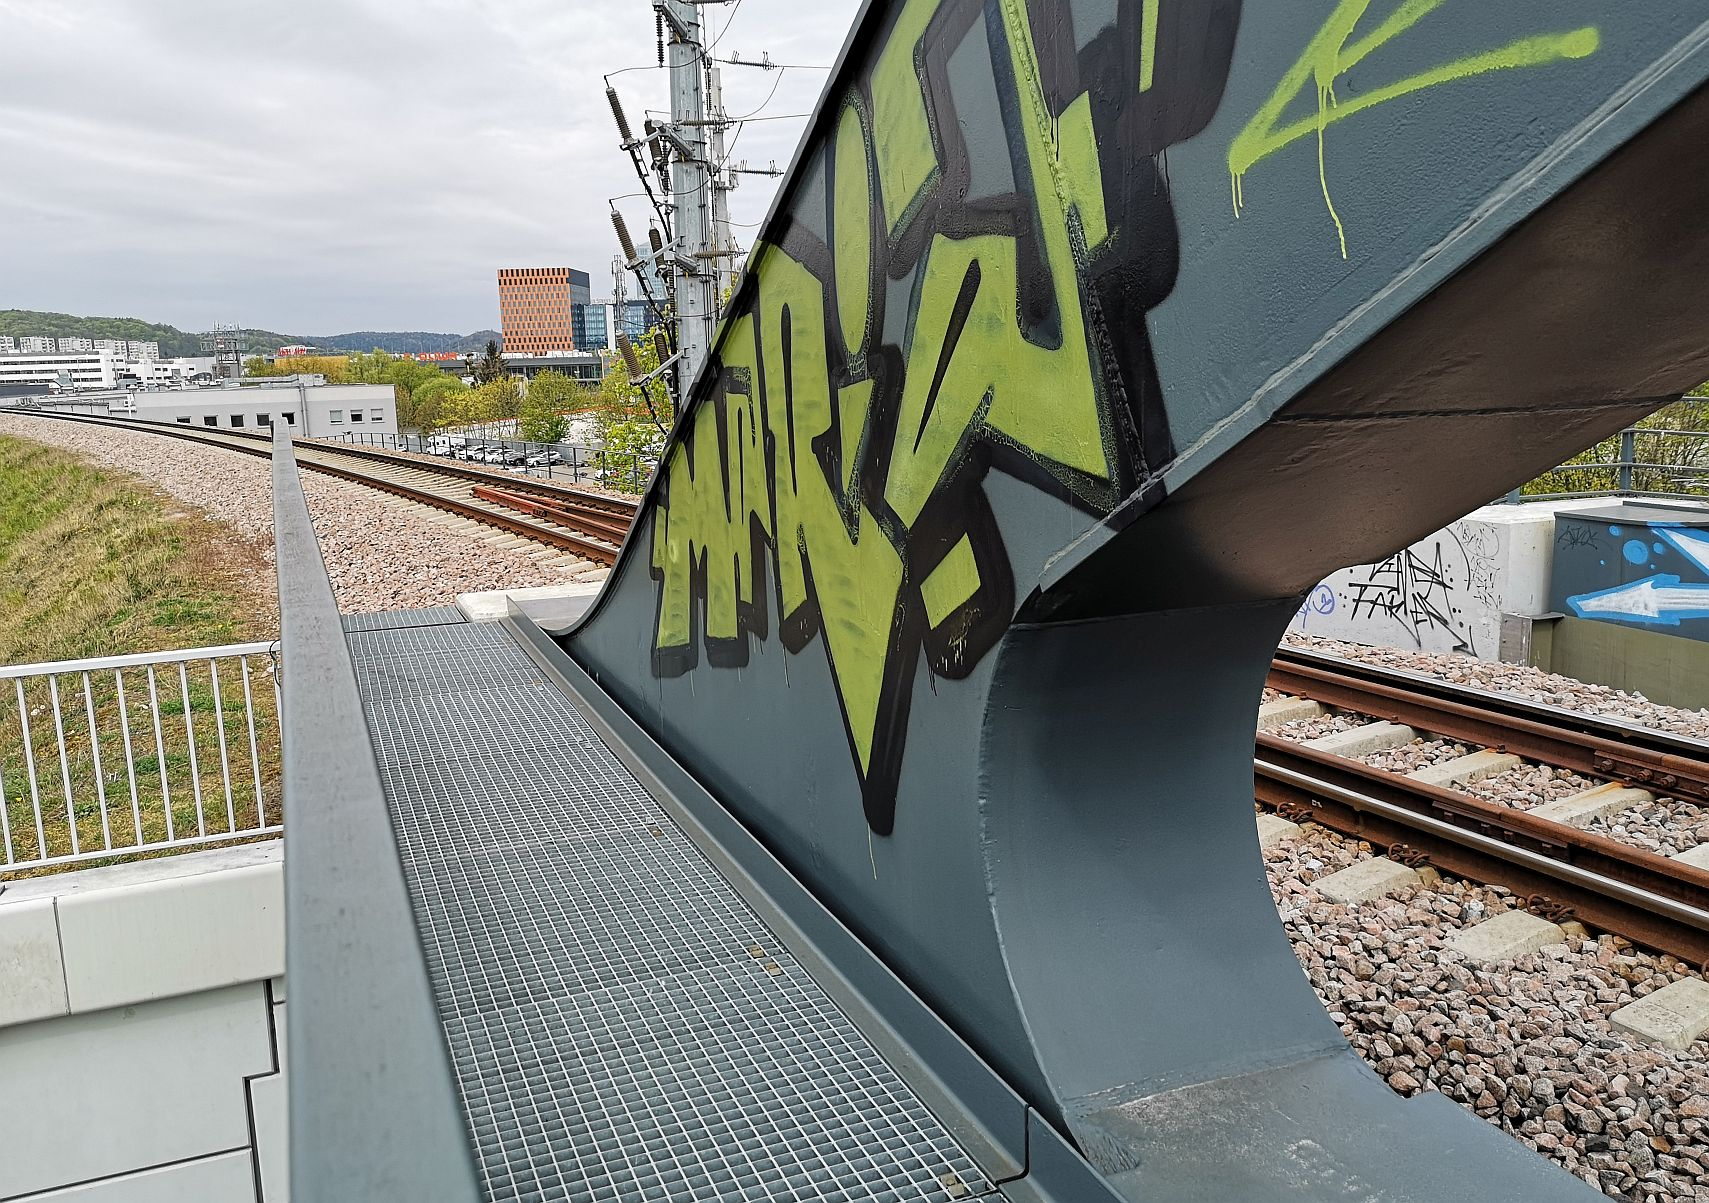
\includegraphics[height=0.2\textheight]{/WK2/zdjecia/wezglowie.jpg}} 
	\qquad
	\subfloat[Widok z dołu]{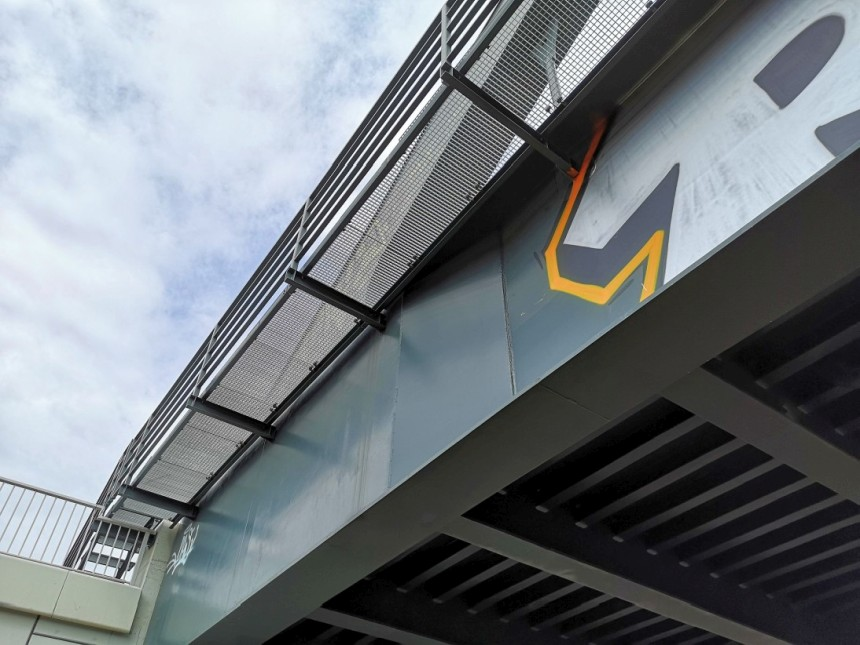
\includegraphics[height=0.2\textheight]{/WK2/zdjecia/detal_wezglowie_dol.jpg}}
	\captionsetup{justification=centering}
	\caption{Szczegóły konstrukcyjne w obrębie połączenia łuku ze ściągiem}
	\label{fig: wk2_foto_wezglowie}
\end{figure}
\begin{figure}[h]
	\centering
	\subfloat{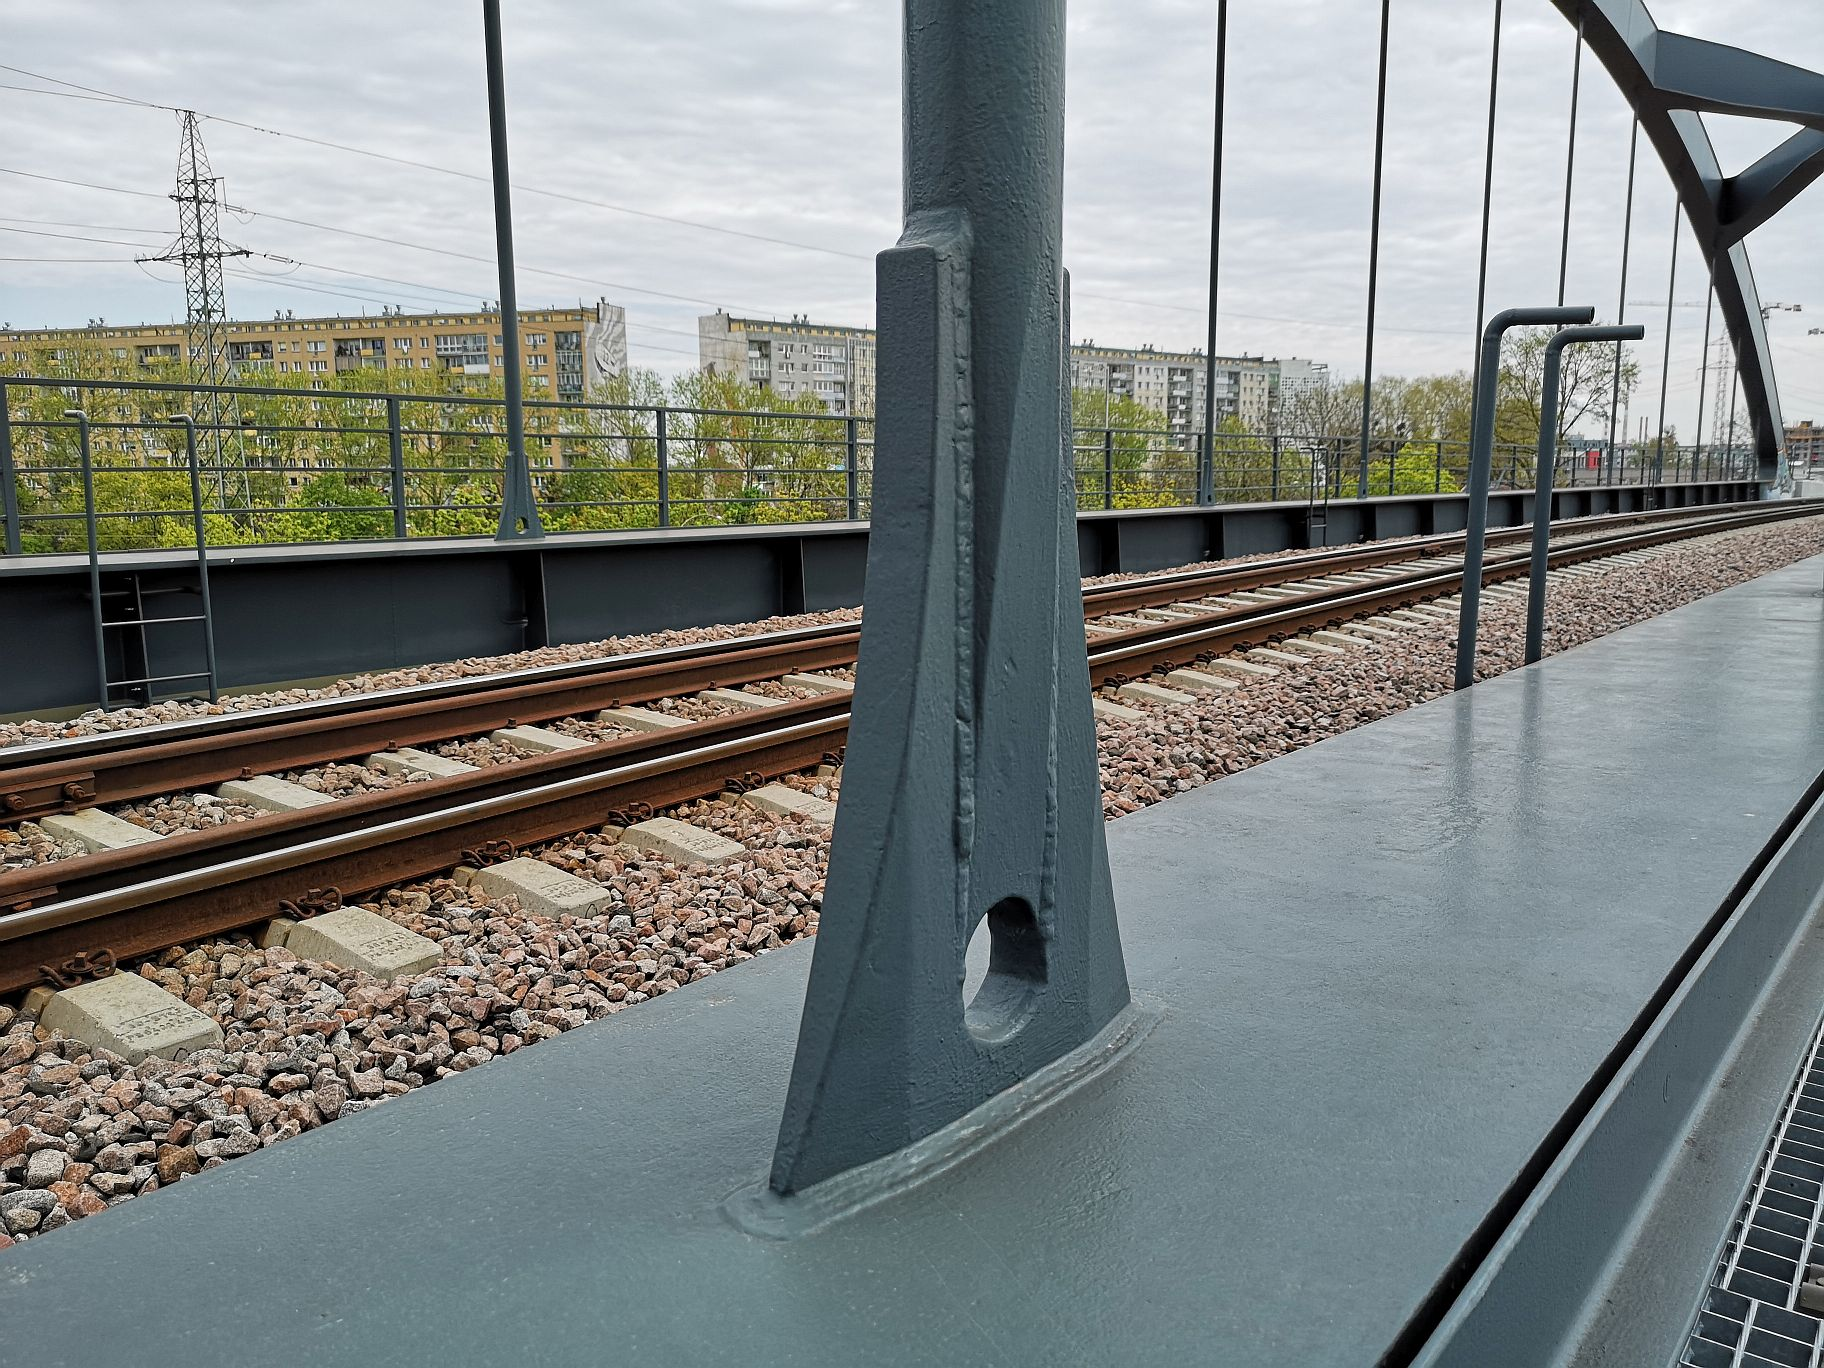
\includegraphics[height=0.2\textheight]{/WK2/zdjecia/zakotwienie_wieszak.jpg}}
	\captionsetup{justification=centering}
	\caption{Detal połączenia wieszaka łuku z pomostem}
	\label{fig: wk2_foto_wieszak}
\end{figure}






\section{Budowa modelu numerycznego}

Na potrzeby analiz numerycznych zbudowano model MES w środowisku SOFiSTiK (rys. \ref{fig: model_wk2_visualization}) Model przestrzenny składa się kilku rodzajów elementów skończonych. Z jednowymiarowych elementów belkowych wykonano łuki, stężenia, belki ściągu, wzmocnienia wezgłowii i żebra pomostu ortotropowego. Z elementów kratowych stworzono wieszaki. Blachę pomostu wykonano z czterowęzłowych elementów powłokowych. Połączenia pomiędzy końcami wieszaków i osiami łuku oraz ściągu zrealizowano przez połączenia kinematyczne translacji i rotacji węzłów. Podparcia pionowe w miejscach łożysk mostu zrealizowano za pomocą sztywnych więzów węzłów. Nie zablokowano przesuwów podłużnych i poprzecznych za pomocą blokady przemieszczeń. Zamiast tego na obu kierunkach zamocowano elastyczne elementy o bardzo dużej sztywności. Dostosowanie do istniejących warunków łożyskowania opisane zostało w dalszej części rozdziału. Usztywnienia wezgłowii zamodelowano za pomocą rusztu elementów belkowych o przekroju składającym się z dwóch blach odsuniętych od siebie na szerokość przekroju skrzynkowego łuku. Elementy strukturalne konstrukcji (takie jak ściągi, pomost, dźwigary łukowe, elementy podparcia itd.) podzielono w modelu na grupy pozwalające odnosić się do nich jako całości. Przekroje elementów belkowych przyjęto zgodnie z dostępną dokumentacją (!!!). Wymiary przekrojów zmiennych po długości zostały interpolowane liniowo. Widoczne na rysunku (\ref{fig: model_wk2_static_scheme}) dodatkowe połączenia kinematyczne są przygotowaniem dla możliwości podłączenia innych konfiguracji wieszaków.



\begin{figure}[h]
	\centering
	\subfloat[Widok A]{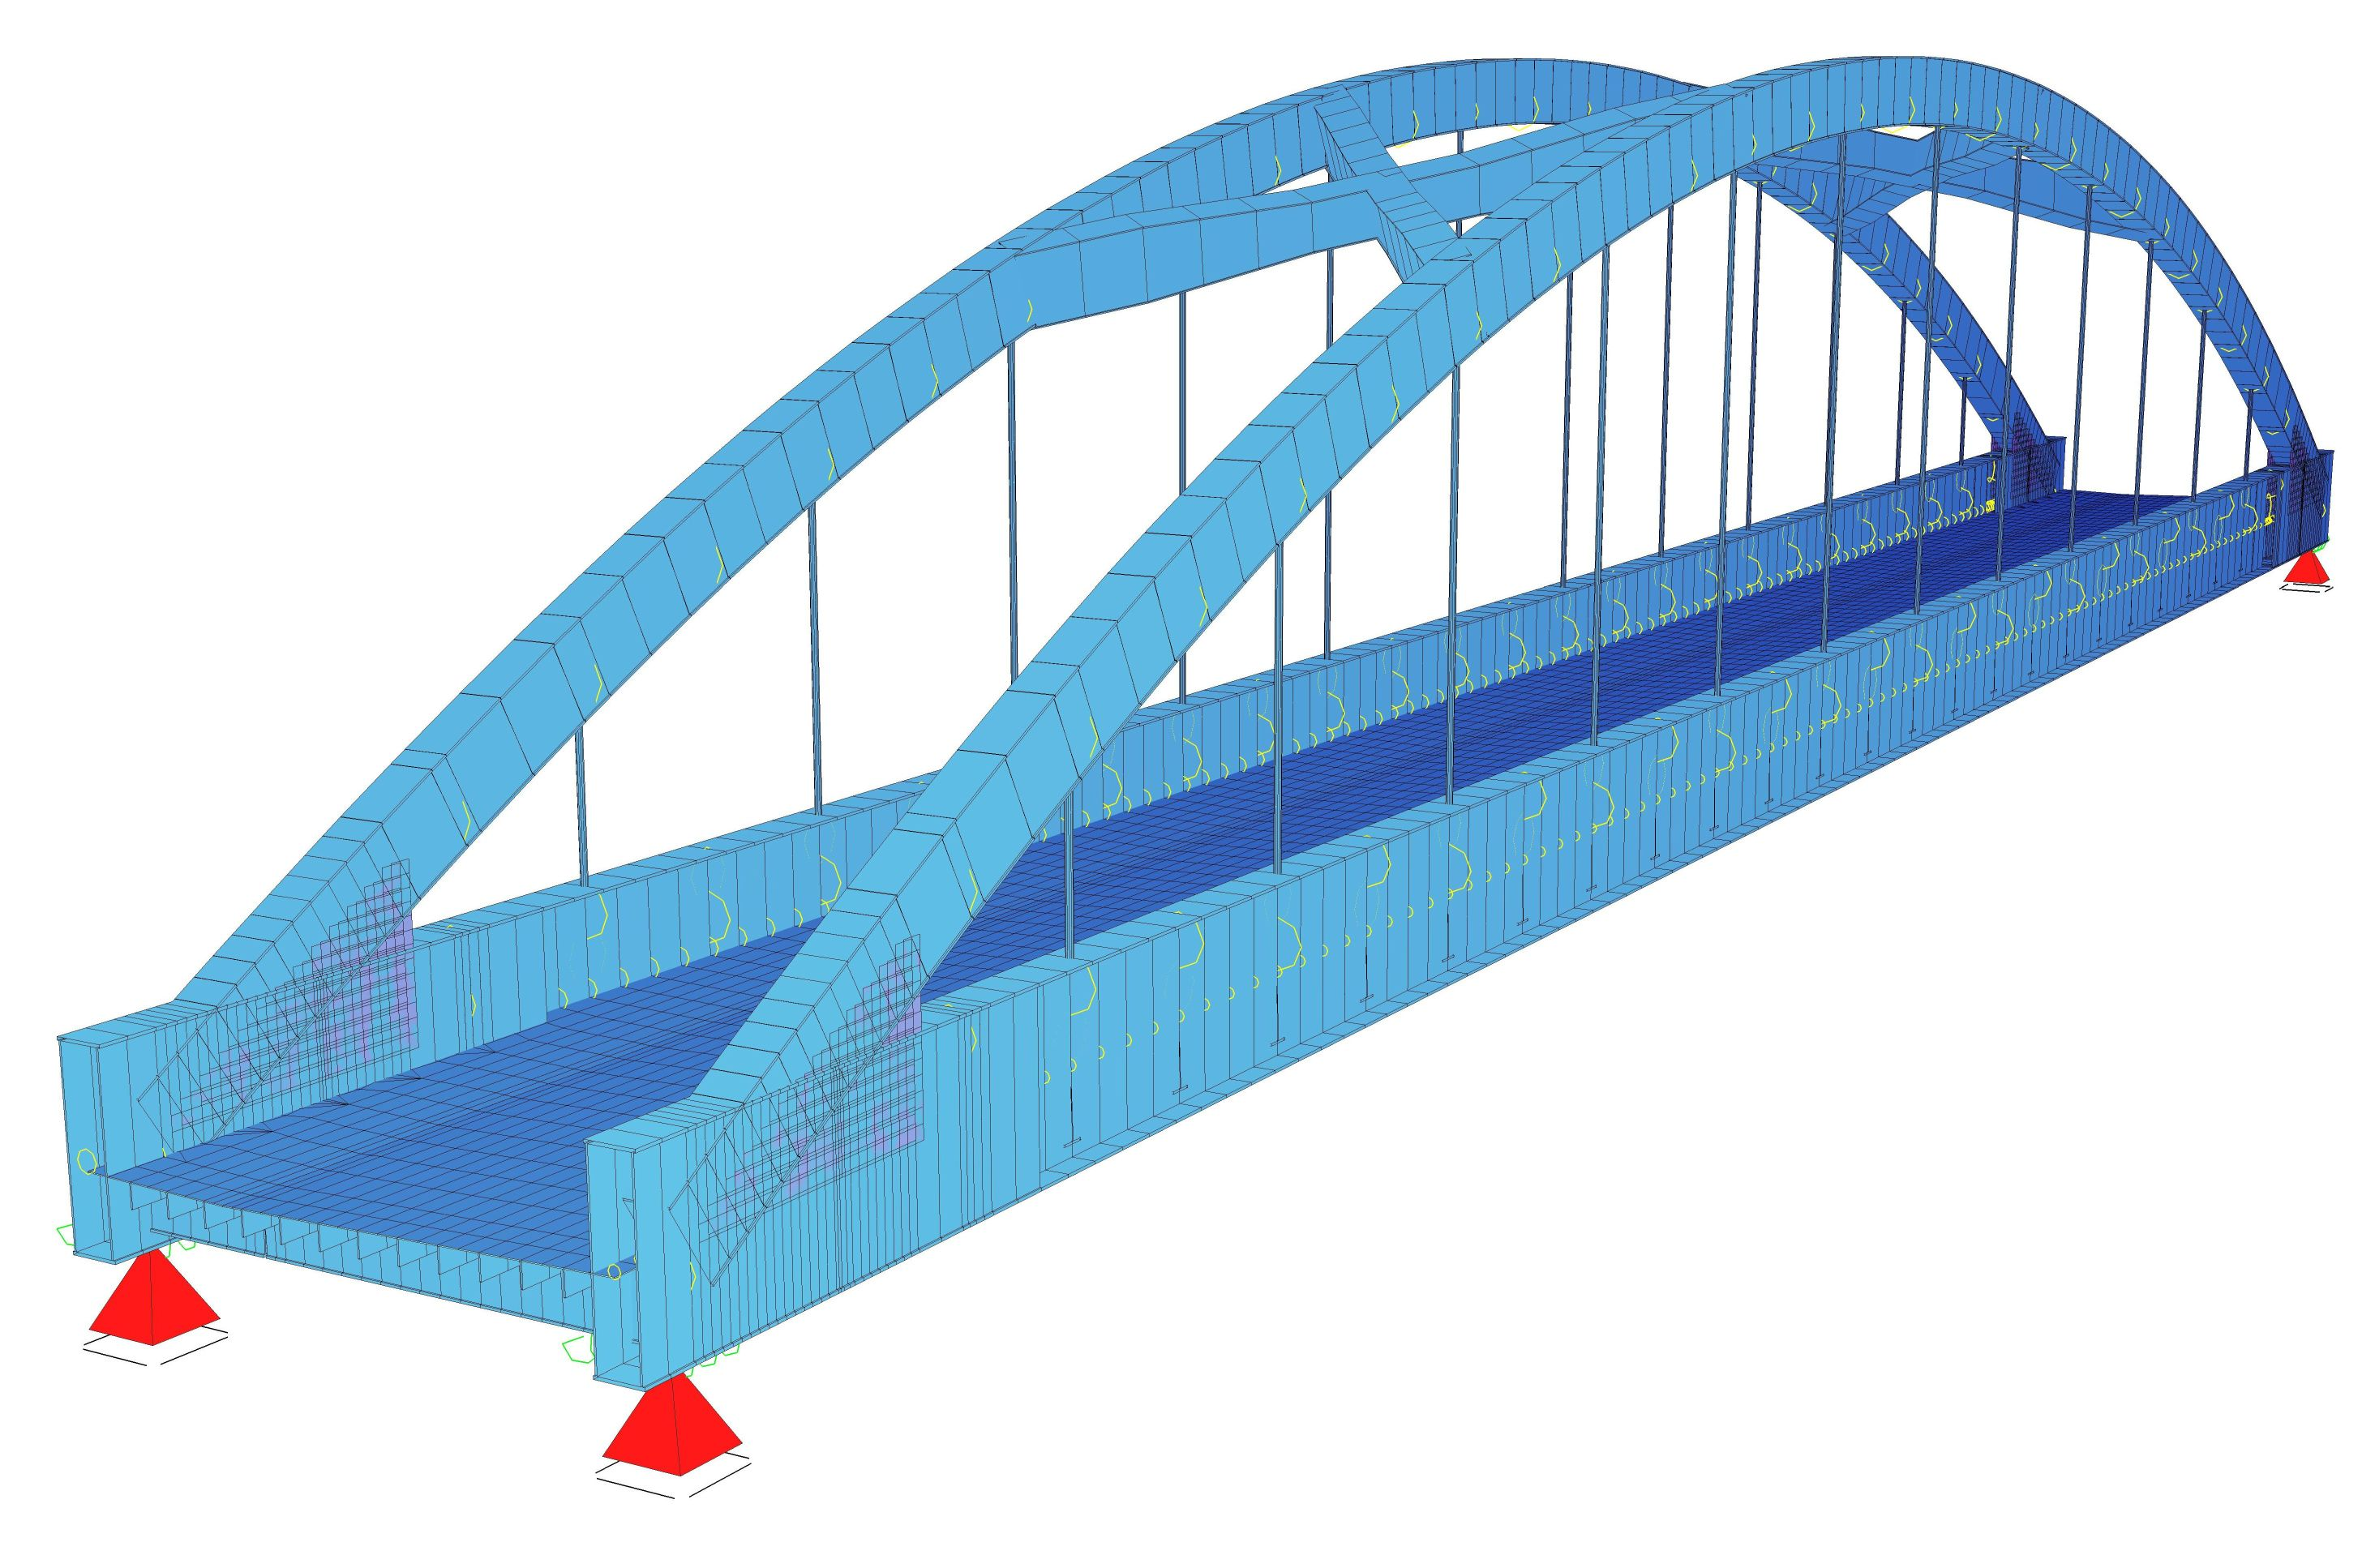
\includegraphics[width=0.5\linewidth]{/WK2/model/SCIAG_PAR_v01_vis_1.jpg}}%
	\subfloat[Widok B]{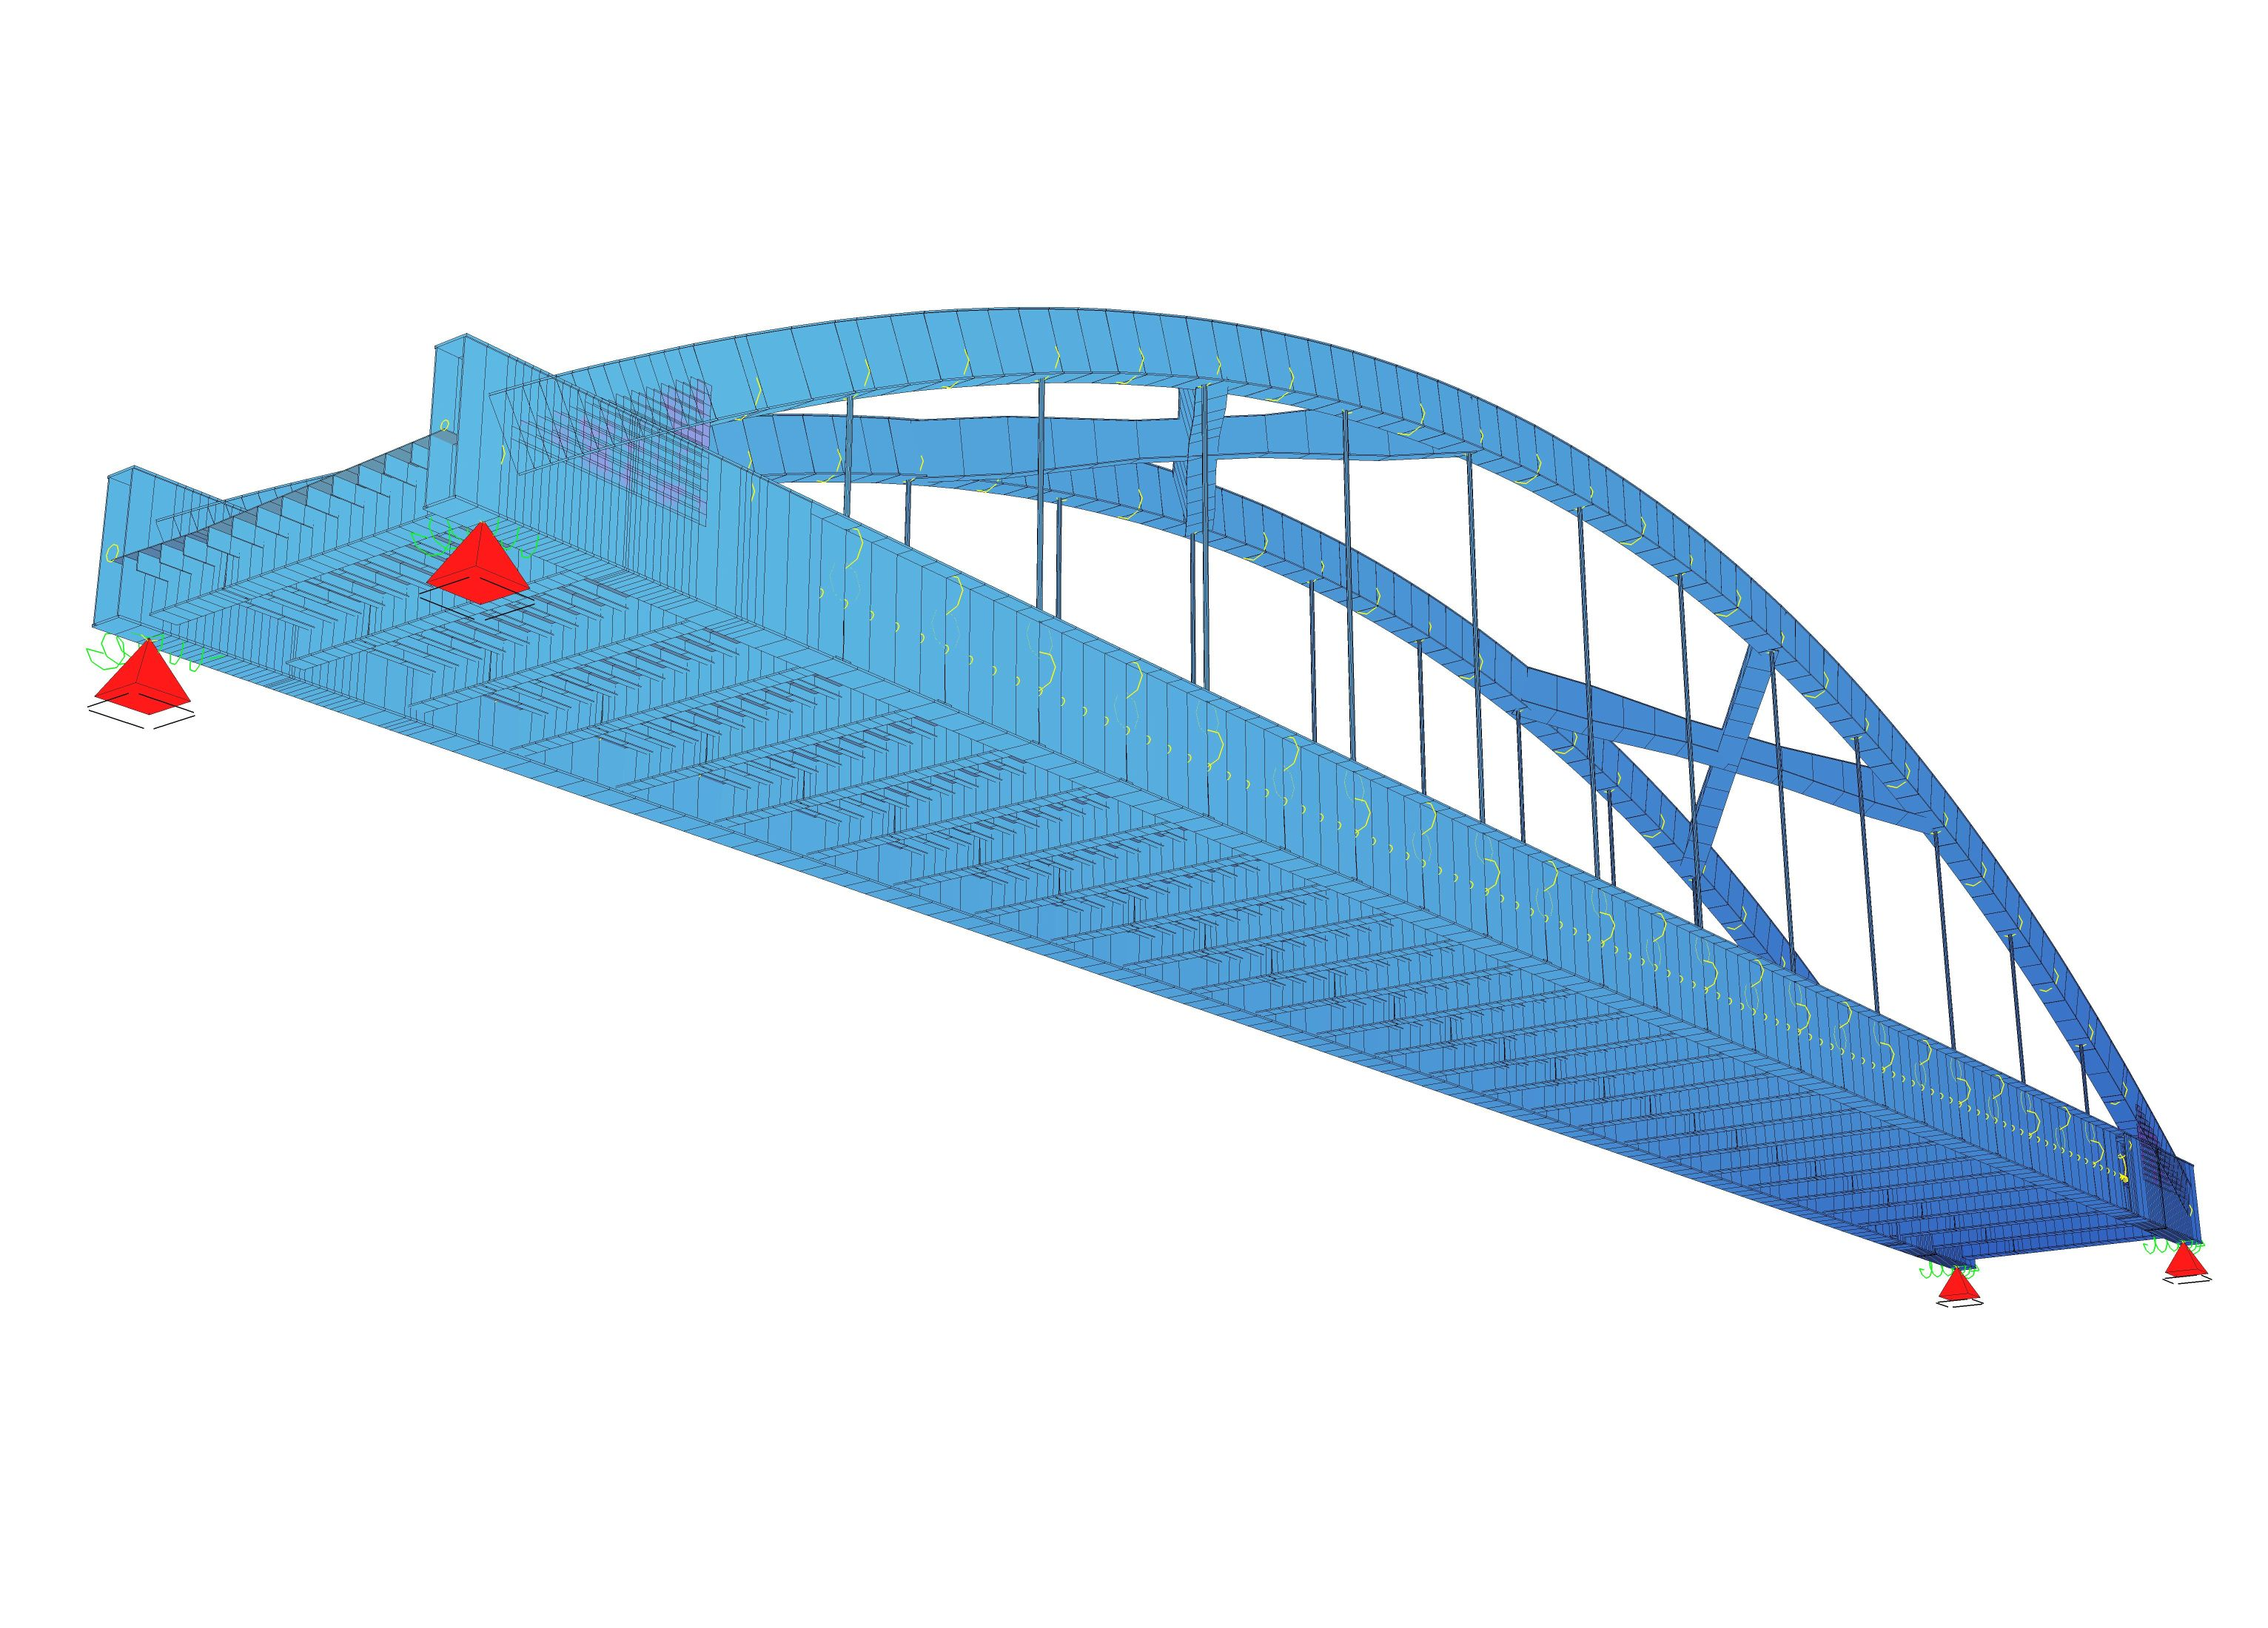
\includegraphics[width=0.5\linewidth]{/WK2/model/SCIAG_PAR_v01_vis_2.jpg}}
	\captionsetup{justification=centering}
	\caption{PODMIENIC NA RZECZYWISTE WYMIARY KONSTRUKCJI!!!!! Wizualizacja przestrzennego modelu numerycznego wiaduktu WK2 Pomorskiej Kolei Metropolitalnej}
	\label{fig: model_wk2_visualization}
	
\end{figure}
\begin{figure}[h]
	\centering
	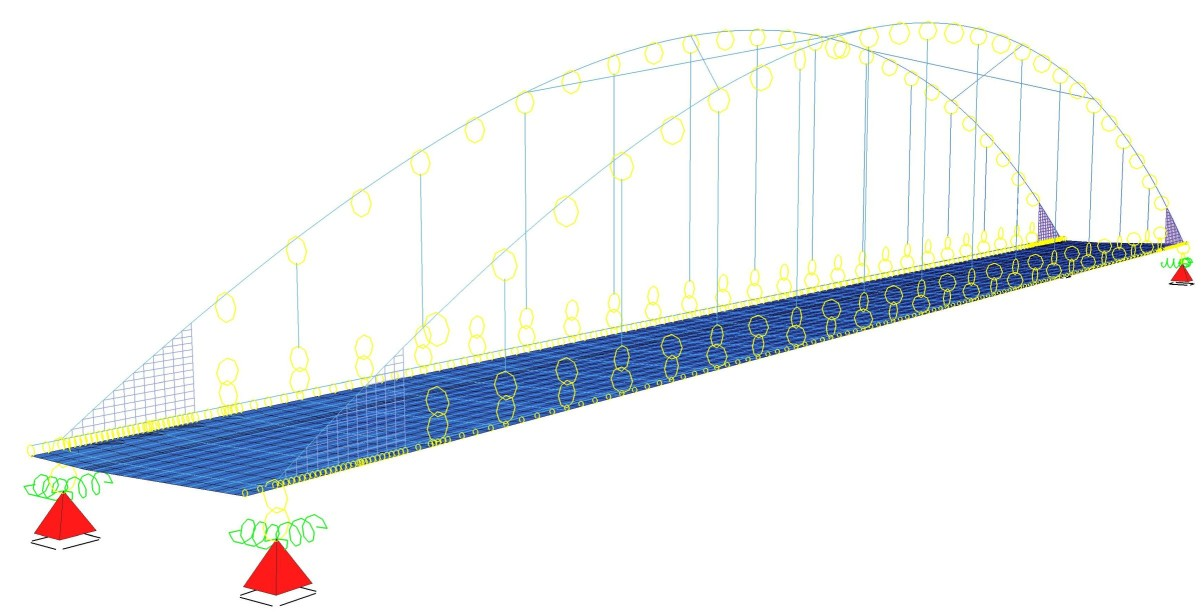
\includegraphics[width=0.8\linewidth]{/WK2/model/SCIAG_PAR_v01_schemat_1.jpg}
	\captionsetup{justification=centering}
	\caption{Schemat statyczny modelu numerycznego wiaduktu WK2 Pomorskiej Kolei Metropolitalnej}
	\label{fig: model_wk2_static_scheme}
\end{figure}

Obciążenie ciężarem własnym konstrukcji zostało wygenerowane na podstawie ciężarów wprowadzonych przekrojów elementów liniowych bądź grubości elementów powłokowych. Dodatkowe elementy takie jak przepony i zakotwienia wieszaków dodane zostały jako obciążenia węzłowe. Osobny przypadek obciążenia stanowi pomost roboczy dodany jako ekwiwalentne obciążenie węzłowe i momenty zginające. Ostatnim obciążeniem stałym jest ciężar tłucznia. Z uwagi na ułożenie toru po łuku w planie, rozkład tłucznia na obiekcie nie jest regularną, symetryczną bryłą. Dostępna dokumentacja obiektu nie dostarcza dokładnych informacji o ułożeniu podsypki na pomoście. Podsypka została w prosty sposób zinwentaryzowana przez pomiar grubości w niektórych punktach charakterystycznych. Jednakże nie jest to precyzyjna metoda i na pewno nie odzwierciedla realnego rozkładu ciężaru podsypki na obiekcie. Z tego względu podzielono obciążenie tłuczniem na dwa osobne przypadki: równomiernie rozłożone obciążenie na całym pomoście i obciążenie równomierne o szerokości (!!!) usytuowane wzdłuż osi toru. Wartość obciążenia tłuczniem przyjęto z normy (!!!).



\section{Badania - identyfikacja modalna: wybór punktów, opis badań, wyniki identyfikacji}
Zastosowane kryteria: max mac 0.6, rowno na obie strony, maksymalna srednia z wektorow punktow. Dodac zmiennosc w kombinacjach maksymalnego momentu jako przestroge.


\begin{figure}[h]
	\centering
	\subfloat[System akwizycji: komputer i wzmacniacz pomiarowy PMX]{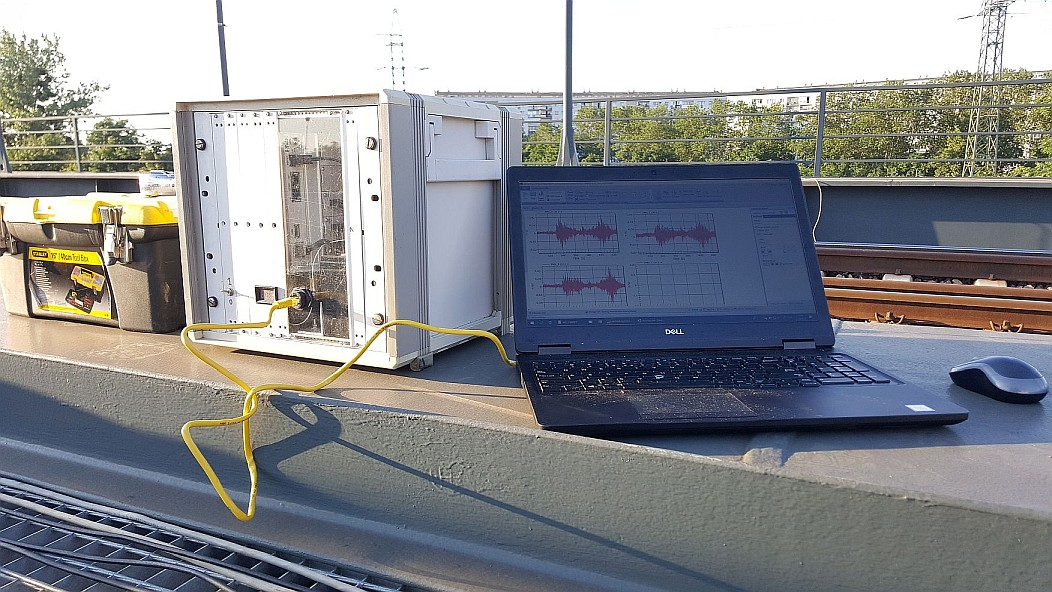
\includegraphics[width=0.48\linewidth]{/WK2/zdjecia/system_pomiarowy.jpg}} \quad 
	\subfloat[3 osiowy akcelerometr]{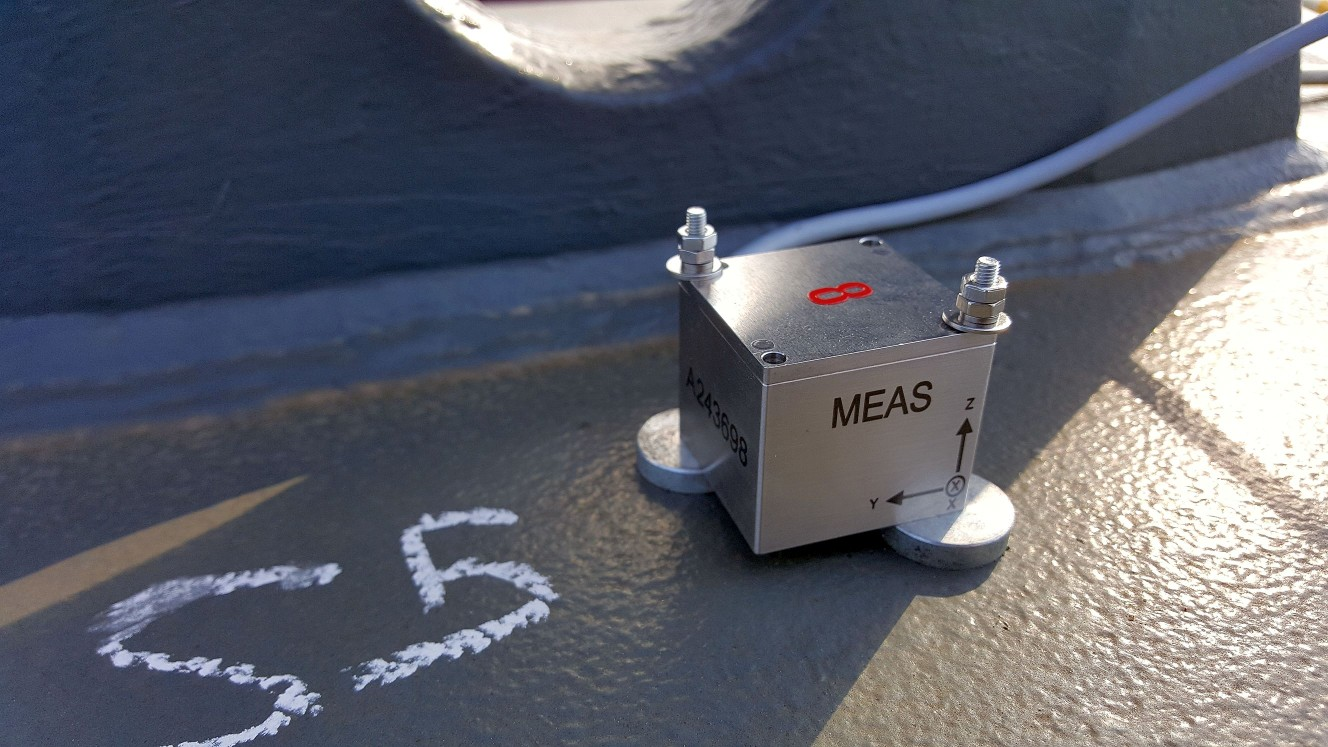
\includegraphics[width=0.48\linewidth]{/WK2/zdjecia/czujnik_3_osie.jpg}} 
	\captionsetup{justification=centering}
	\caption{System pomiarowy użyty do identyfikacji modalnej wiaduktu WK2}
	\label{fig: wk2_foto_aparatura}
\end{figure}



\begin{figure}[h]
	\centering
	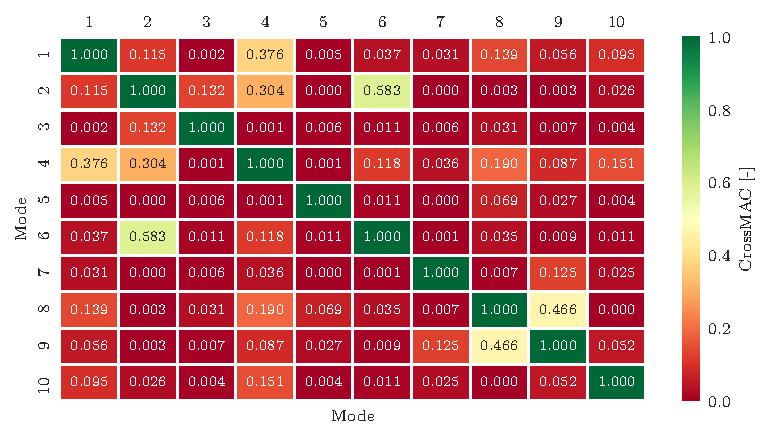
\includegraphics[width=\textwidth]{WK2/correlogram_badania.pdf}
	\captionsetup{justification=centering}
	\caption{Diagram AUTOMAC dla pierwszych dziesięciu wektorów postaci drgań własnych, odczytanych z modelu dla wybranych punktów pomiarowych}
\end{figure}
\begin{figure}[h]
	\centering
	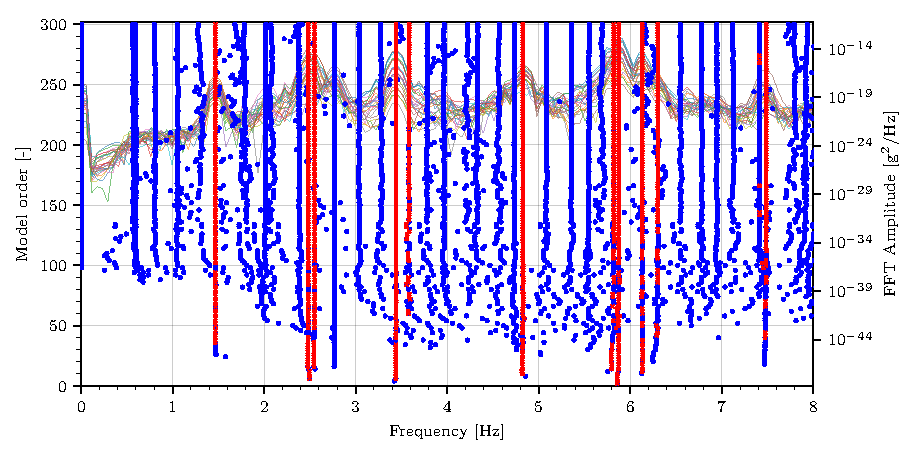
\includegraphics[width=\textwidth]{WK2/diagram_non_filtered.pdf}
	\captionsetup{justification=centering}
	\caption{Diagram stabilizacyjny metody NExT-ERA.}
\end{figure}
\begin{figure}[h]
	\centering
	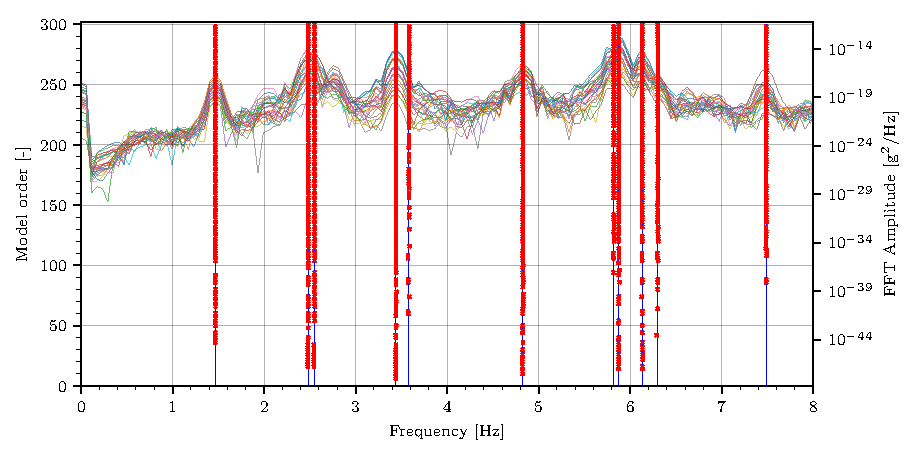
\includegraphics[]{WK2/diagram_filtered2.pdf}
	\captionsetup{justification=centering}
	\caption{Diagram stabilizacyjny metody NExT-ERA.}
\end{figure}
\begin{figure}[h]
	\centering
	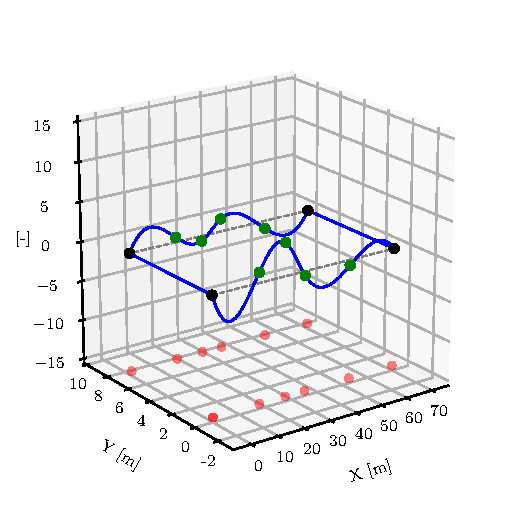
\includegraphics[]{WK2/identified_mode_1.pdf}
	\captionsetup{justification=centering}
	\caption{Diagram stabilizacyjny metody NExT-ERA.}
\end{figure}

\section{Kalibracja modelu numerycznego z wykorzystaniem PSO}
\section{Wielokryterialna optymalizacja modelu: opis + wyniki}
\chapter{Podsumowanie i wnioski}
Podsumowania wnioski